\section{Messaggi d'errore} \label{err}
Durante l'utilizzo dell'applicazione \Premi c'è la possibilità che si verifichino degli errori.\\
Questi vengono gestiti dall'applicazione fornendo all'utente un messaggio che lo informa sulla tipologia e sulla causa del malfunzionamento.\\
In seguito verranno elencati gli errori che possono essere sollevati dall'applicazione.
\subsection{Lista degli errori}
La lista che segue contiene il tipo di errore e la sua descrizione per gli errori specifici dell'applicazione \Premi.
\begin{itemize}
\item \texttt{Utente non trovato}: l'identificativo utente fornito non è un identificativo valido;
\item \texttt{Credenziali non valide}: è necessario fornire un indirizzo email ed una password valide;
\item \texttt{\gloxy{Progetto} non trovato}: l'identificativo del \gloxy{progetto} fornito non è un identificativo valido;
\item \texttt{Nodo non trovato}: l'identificativo del nodo fornito non è un identificativo valido;
\item \texttt{Associazione non trovata}: l'identificativo dell'associazione fornita non è un identificativo valido;
\item \texttt{\gloxy{Percorso} non trovato}: l'identificativo del \gloxy{percorso} fornito non è un identificativo valido;
\item \texttt{\gloxy{Progetto} corrotto}: errore nella ricerca dei campi dati relativi al \gloxy{progetto} indicato;
\item \texttt{Dati non validi}: i dati relativi al \gloxy{progetto} sono vuoti o errati;
\item \texttt{\gloxy{Progetto} corrotto}: errore durante l'eliminazione del \gloxy{progetto};
\item \texttt{Dati non validi}: i dati relativi al contenuto del nodo non sono validi o sono formattati in modo errato;
\item \texttt{Nodi non validi}: gli identificativi dei nodi forniti non sono validi oppure non esistono oppure il nodo entrante coincide con il nodo uscente;
\item \texttt{Dati non validi}: i dati per la modifica del \gloxy{percorso} non sono definiti;
\item \texttt{Nodo del \gloxy{progetto} non trovato}: il nodo riferito nella relazione o nel \gloxy{percorso} non è stato trovato all'interno del \gloxy{progetto} indicato;
\item \texttt{Nodo padre non esistente}: il nodo padre indicato non esiste o non corrisponde ad un nodo valido;
\item \texttt{Nodo non valido}: impossibile eliminare il nodo radice della mappa mentale.
\item \texttt{Nodo del \gloxy{percorso} non trovato}: il nodo riferito non è stato trovato all'interno del \gloxy{percorso} indicato.
\end{itemize}
Gli errori vengono segnalati all'utente tramite la visualizzazione di un \textit{popup}, in cui è presente la descrizione dell'errore.
\begin{figure}[H]
\centering
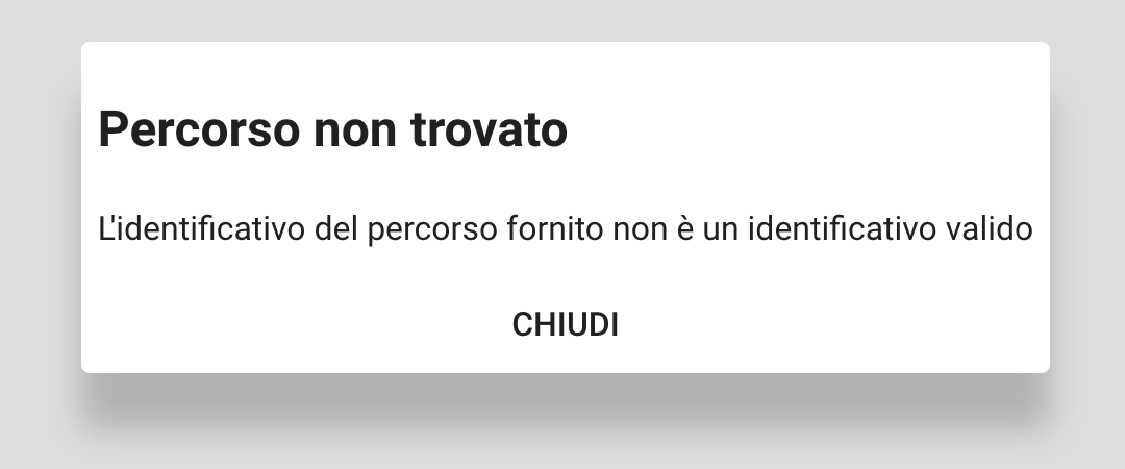
\includegraphics[scale=0.5]{immagini/errore.pdf}
\caption{Popup di notifica errore}
\end{figure}
Nel caso in cui l'utente desideri segnalare la presenza di errori non segnalati o ricevere informazioni specifiche riguardo agli errori dell'applicazione, può contattare il \gloxy{team} seguendo le indicazioni presenti nella sezione \textit{\nameref{sgnErr}}.
